\documentclass[12pt,a4paper]{article}
\usepackage[T2A]{fontenc}
\usepackage[utf8]{inputenc}
\usepackage[russian]{babel}
\usepackage{amsmath, amssymb, amsfonts}
\usepackage{geometry}
\usepackage{graphicx}
\usepackage{float}
\usepackage{booktabs}
\usepackage{array}
\usepackage{longtable}
\usepackage{listings}
\usepackage{xcolor}
\usepackage{hyperref}
\usepackage{indentfirst}
\usepackage{setspace}

\geometry{
    left=30mm,
    right=15mm,
    top=20mm,
    bottom=20mm
}
\onehalfspacing

\hypersetup{
    colorlinks=true,
    linkcolor=black,
    urlcolor=black,
    citecolor=black
}

\lstdefinestyle{codestyle}{
    basicstyle=\ttfamily\small,
    breaklines=true,
    frame=single,
    numbers=left,
    numberstyle=\tiny,
    keywordstyle=\bfseries,
    commentstyle=\itshape,
    showstringspaces=false,
    tabsize=4,
    captionpos=b
}
\lstset{style=codestyle}

\begin{document}

\begin{titlepage}
\begin{center}
Федеральное государственное автономное образовательное учреждение высшего образования\\
«Национальный исследовательский университет ИТМО»
\end{center}

\vspace{1cm}
\begin{center}
Факультет технологий искусственного интеллекта
\end{center}

\vfill
\begin{center}
{\Large Лабораторная работа №1}\\[0.4cm]
{\large Численное решение задачи Коши для уравнения первого порядка}
\end{center}
\vfill

\begin{flushright}
Выполнил:\\
студент группы J3210\\
Тищенко Павел\\[0.8cm]
Проверил:\\
преподаватель\\
\underline{\hspace{4cm}}
\end{flushright}

\vfill
\begin{center}
Санкт-Петербург\\
2026
\end{center}
\end{titlepage}

\tableofcontents
\newpage

\section{Цель работы}
Исследовать численное решение задачи Коши для ОДУ первого порядка методами Эйлера, Хойна и Рунге--Кутты 4-го порядка, сравнить численные решения с аналитическим и оценить абсолютную и относительную погрешности.

\section{Постановка задачи}
Для варианта 6 требуется решить задачу:
\[
y' = f(x,y), \quad y(x_0)=y_0, \quad x\in[x_0,b],
\]
\[
f(x,y)=\frac{1}{x^2+x+1}-\frac{y}{x+0.5}, \quad y(0)=1.
\]
Выбранные параметры интегрирования:
\[
x_0=0,\quad b=2,\quad n=200,\quad h=\frac{b-x_0}{n}=0.01.
\]

\section{Теоретическая часть}
\subsection{Задача Коши и сетка}
Используется равномерная сетка:
\[
x_k=x_0+kh,\quad k=0,\dots,n,\quad h=\frac{b-x_0}{n}.
\]

\subsection{Метод Эйлера}
\[
y_{k+1}=y_k+h f(x_k,y_k).
\]

\subsection{Метод Хойна}
\[
\hat y_{k+1}=y_k+h f(x_k,y_k),
\]
\[
y_{k+1}=y_k+\frac{h}{2}\left(f(x_k,y_k)+f(x_{k+1},\hat y_{k+1})\right).
\]

\subsection{Метод Рунге--Кутты 4-го порядка}
\[
k_1=f(x_k,y_k),\qquad
k_2=f\left(x_k+\frac{h}{2},y_k+\frac{h k_1}{2}\right),
\]
\[
k_3=f\left(x_k+\frac{h}{2},y_k+\frac{h k_2}{2}\right),\qquad
k_4=f(x_k+h,y_k+h k_3),
\]
\[
y_{k+1}=y_k+\frac{h}{6}(k_1+2k_2+2k_3+k_4).
\]

\subsection{Формулы погрешностей}
\[
\Delta_l=\max_{k=1,\ldots,n}\left|\varphi(x_k)-\widetilde{\varphi}_l(x_k)\right|,
\]
\[
\delta_l=\max_{k=1,\ldots,n}
\frac{\left|\varphi(x_k)-\widetilde{\varphi}_l(x_k)\right|}
{\left|\widetilde{\varphi}_l(x_k)\right|}.
\]

\section{Аналитическое решение}
Перепишем уравнение:
\[
y' + \frac{1}{x+0.5}y=\frac{1}{x^2+x+1}.
\]
Интегрирующий множитель:
\[
\mu(x)=\exp\left(\int\frac{dx}{x+0.5}\right)=x+0.5.
\]
Тогда
\[
\frac{d}{dx}\left((x+0.5)y\right)=\frac{x+0.5}{x^2+x+1}
=\frac{1}{2}\frac{2x+1}{x^2+x+1}.
\]
После интегрирования:
\[
(x+0.5)y=\frac{1}{2}\ln(x^2+x+1)+C.
\]
Из $y(0)=1$ получаем $C=0.5$, поэтому
\[
\varphi(x)=\frac{0.5\ln(x^2+x+1)+0.5}{x+0.5}.
\]

\section{Программная реализация}
Программная часть выполнена на C\# (численные методы, расчёт ошибок) и Python (построение графиков и формирование таблиц для отчёта). Полный исходный код доступен в репозитории:

\begin{center}
\url{https://github.com/paulhowever/diff_labs}
\end{center}

Основные файлы ЛР1:
\begin{itemize}
\item \texttt{lab1/src/Lab1.Core/Variants/Lab1Variant6.cs} --- постановка варианта и аналитическое решение;
\item \texttt{lab1/src/Lab1.Core/Methods/*.cs} --- Эйлер, Хойн, RK4;
\item \texttt{lab1/src/Lab1.Core/Solvers/FirstOrderSolver.cs} --- общий проход по сетке и расчёт ошибок;
\item \texttt{reports/lab1/build\_assets.py} --- графики и таблицы для отчёта.
\end{itemize}

Ключевая общая схема одношагового метода:
\begin{lstlisting}[language=Python, caption={Общая схема одношагового численного метода}]
xs = build_uniform_grid(x0, b, n)
ys[0] = y0

for k in range(n):
    ys[k + 1] = next_value(xs[k], ys[k], h, f)
\end{lstlisting}

Функция \texttt{next\_value} задаётся формулами Эйлера, Хойна или RK4 из раздела теории.

\section{Результаты вычислений}
\subsection{Параметры расчёта}
\begin{table}[H]
\centering
\begin{tabular}{lc}
\toprule
Параметр & Значение \\
\midrule
$x_0$ & 0 \\
$b$ & 2 \\
$n$ & 200 \\
$h$ & 0.01 \\
\bottomrule
\end{tabular}
\caption{Параметры численного эксперимента для ЛР1}
\label{tab:lab1_params}
\end{table}

\subsection{Таблица погрешностей}
\begin{table}[H]
\centering
\begin{tabular}{lcc}
\toprule
Метод & $\Delta_l$ & $\delta_l$ \\
\midrule
Euler & 2.659478e-03 & 3.338048e-03 \\
Heun & 4.876432e-06 & 6.220303e-06 \\
RungeKutta4 & 6.223577e-12 & 8.826949e-12 \\
\bottomrule
\end{tabular}
\caption{Максимальные ошибки по методам}
\label{tab:lab1_errors}
\end{table}

\subsection{Сравнение значений в отдельных точках}
\begin{table}[H]
\centering
\begin{tabular}{cccccc}
\toprule
$x_k$ & $\varphi(x_k)$ & Euler & Heun & RK4 & $|e_{RK4}|$ \\
\midrule
0.000 & 1.000000 & 1.000000 & 1.000000 & 1.000000 & 0.000e+00 \\
0.500 & 0.779808 & 0.777218 & 0.779803 & 0.779808 & 3.893e-12 \\
1.000 & 0.699537 & 0.697517 & 0.699534 & 0.699537 & 6.174e-12 \\
1.500 & 0.639536 & 0.637920 & 0.639533 & 0.639536 & 5.180e-12 \\
2.000 & 0.589182 & 0.587817 & 0.589180 & 0.589182 & 4.207e-12 \\
\bottomrule
\end{tabular}
\caption{Сравнение точного и численных решений в узлах сетки}
\label{tab:lab1_points}
\end{table}

\section{Графики решений}
На рисунке~\ref{fig:lab1_solutions} показаны аналитическое и численные решения. На рисунке~\ref{fig:lab1_errors} приведены абсолютные ошибки в логарифмической шкале.

\begin{figure}[H]
\centering
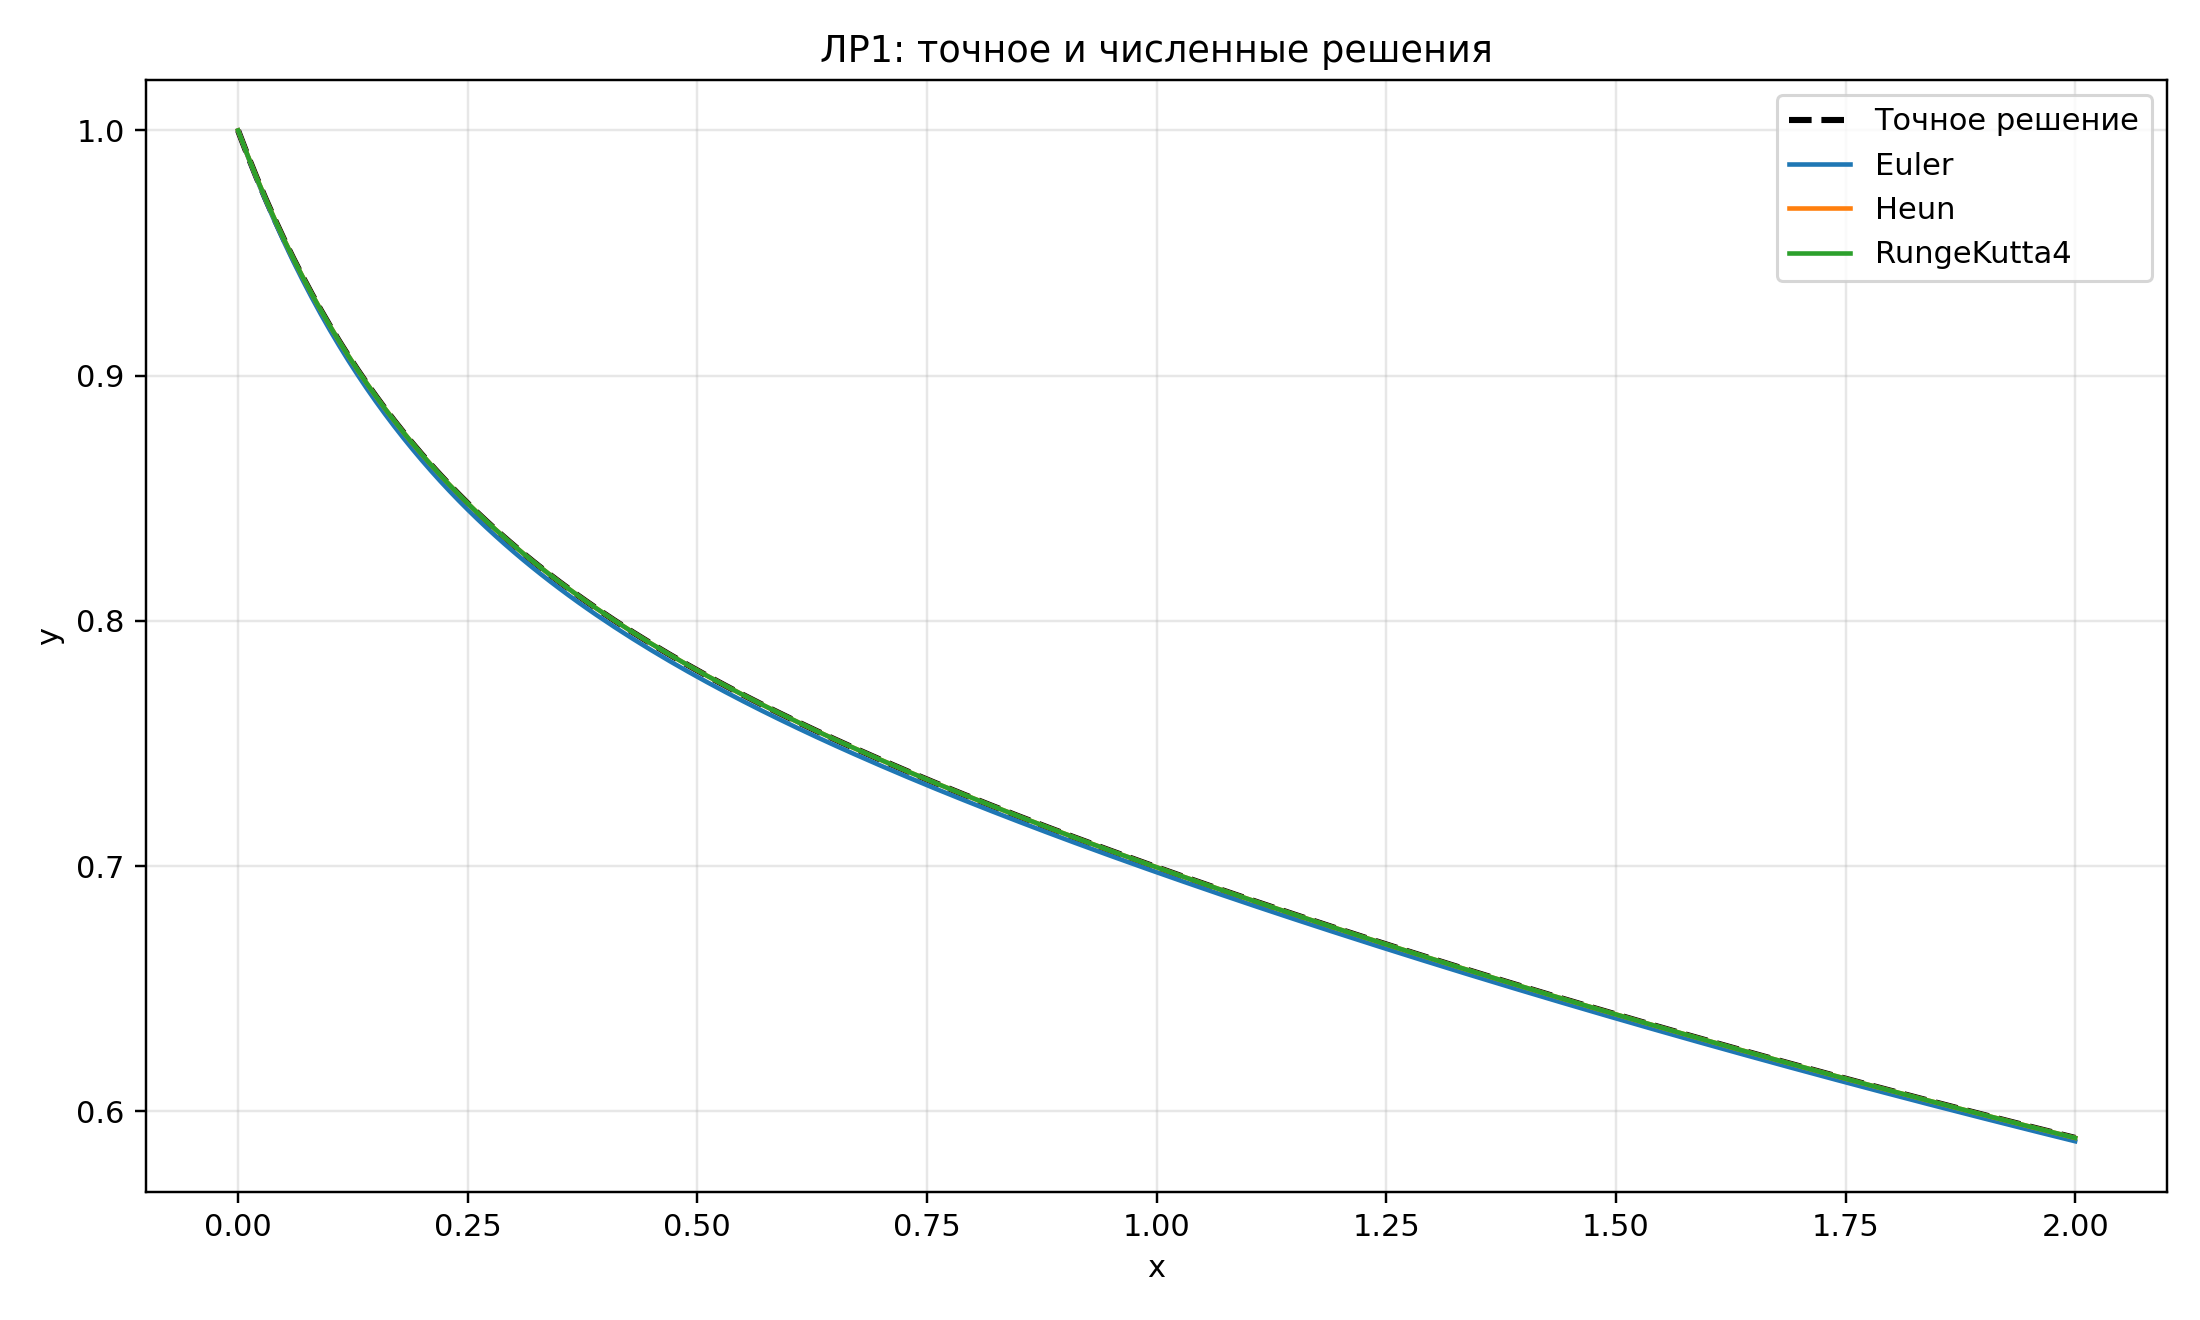
\includegraphics[width=0.92\textwidth]{images/solutions.png}
\caption{Точное и численные решения для ЛР1}
\label{fig:lab1_solutions}
\end{figure}

\begin{figure}[H]
\centering
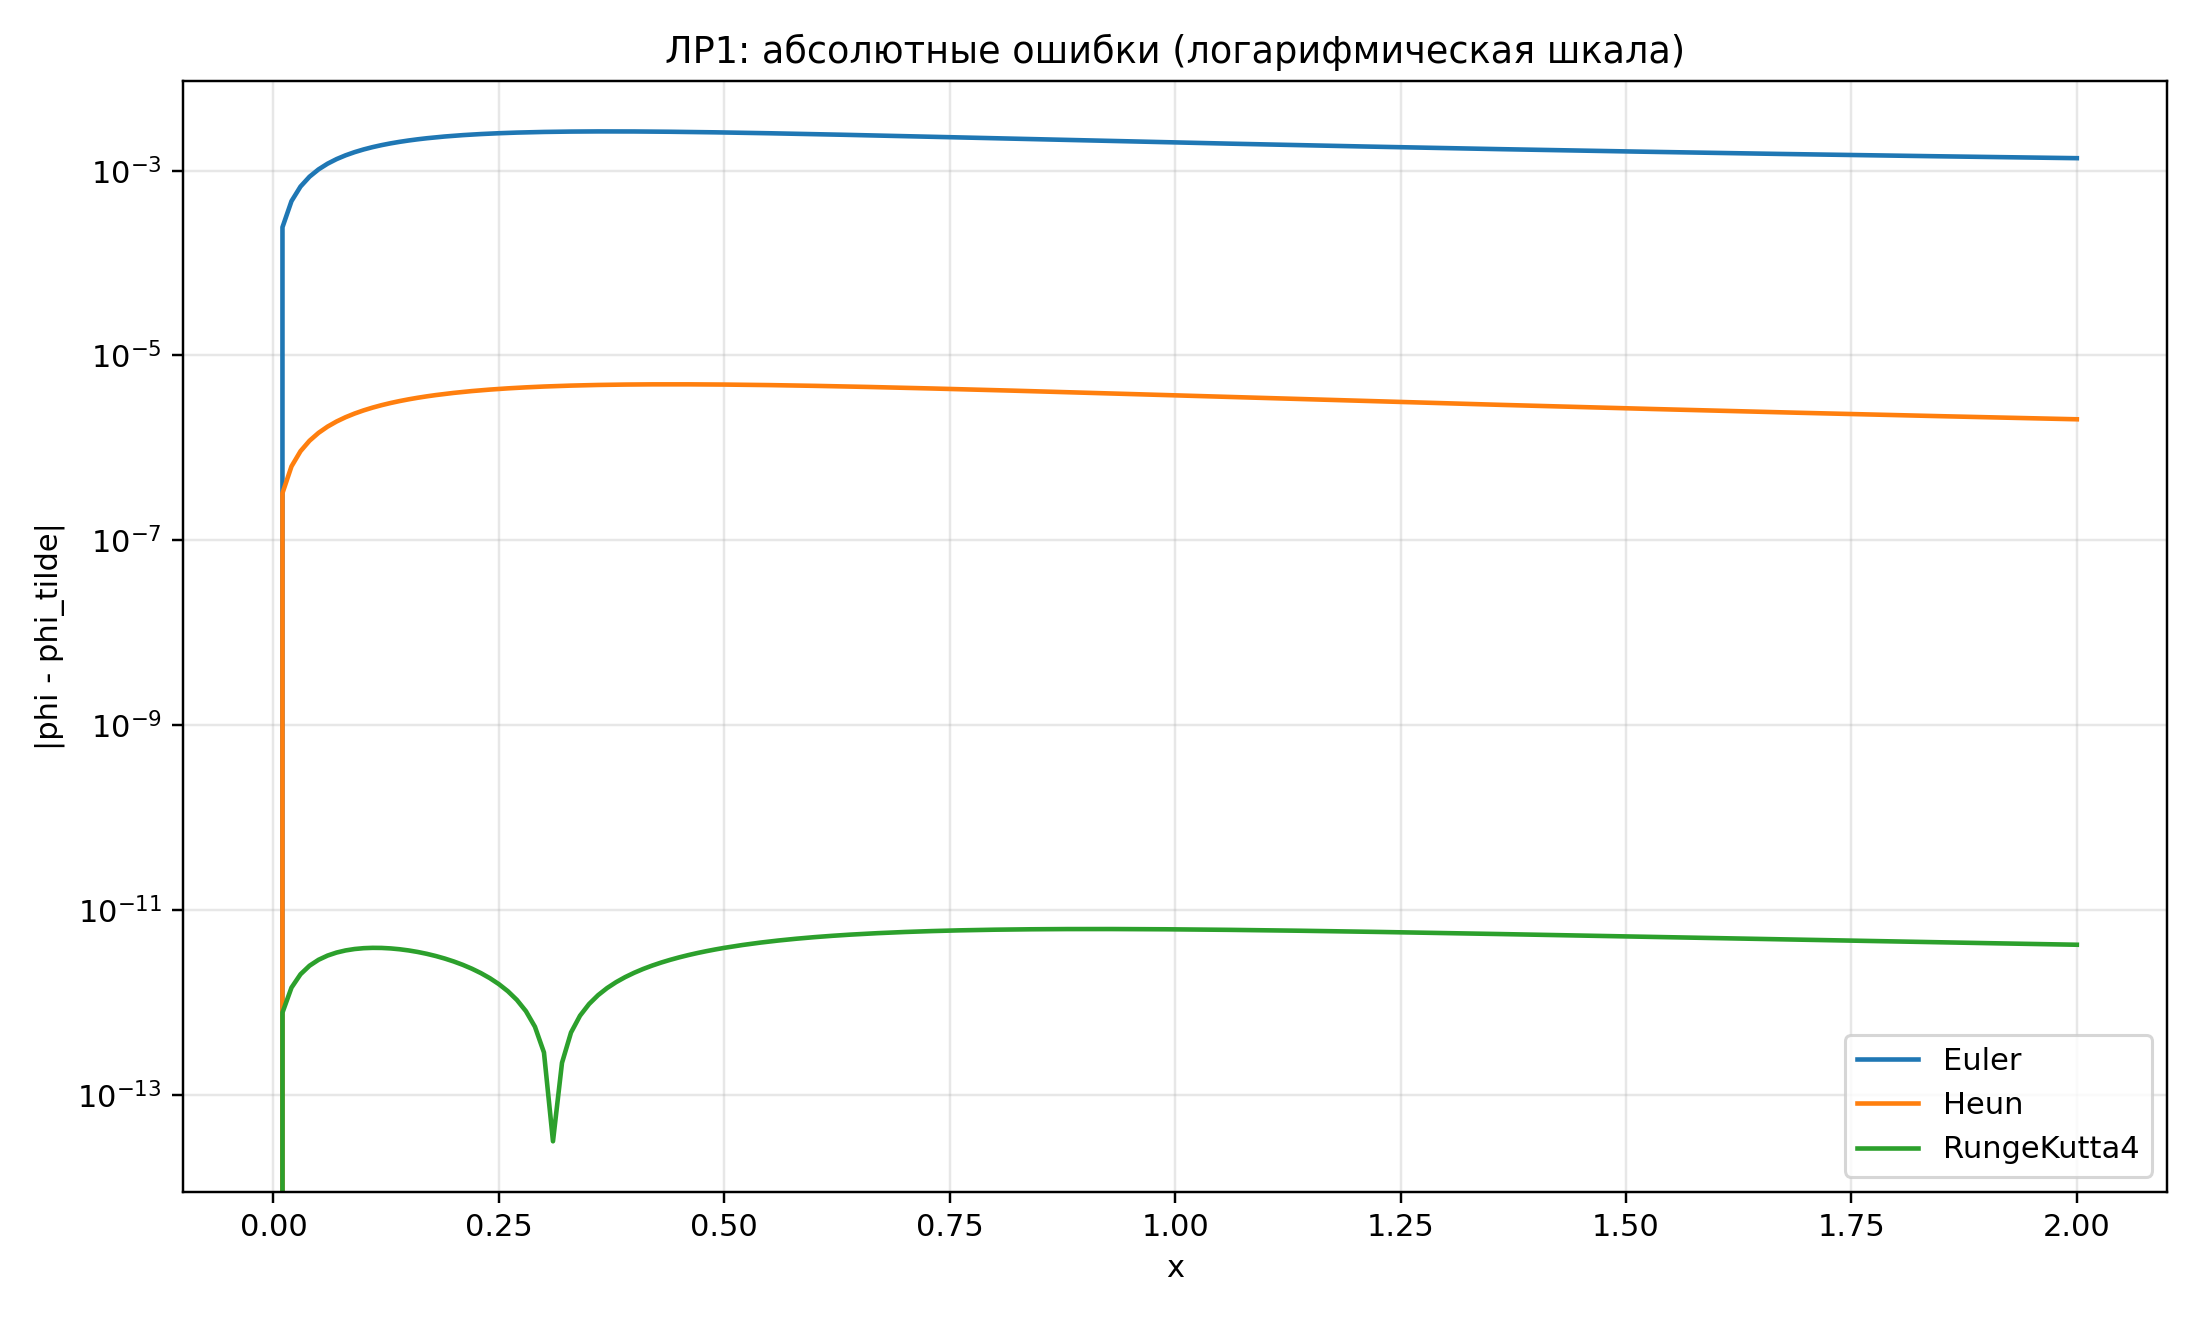
\includegraphics[width=0.92\textwidth]{images/errors.png}
\caption{Абсолютные ошибки методов для ЛР1}
\label{fig:lab1_errors}
\end{figure}

\section{Анализ результатов}
По таблице~\ref{tab:lab1_errors} и рисунку~\ref{fig:lab1_errors} видно ожидаемое распределение точности:
\[
\text{RK4} \succ \text{Хойн} \succ \text{Эйлер}.
\]
Метод Эйлера имеет наибольшую ошибку из-за первого порядка точности. Метод Хойна значительно точнее за счёт предиктор-корректорной схемы. Метод RK4 демонстрирует минимальную ошибку на выбранной сетке и наилучшее совпадение с аналитическим решением на рисунке~\ref{fig:lab1_solutions}.

\section{Вывод}
Задача Коши варианта 6 для уравнения первого порядка решена тремя численными методами при постоянном шаге. Получено аналитическое решение, построены графики и рассчитаны абсолютные и относительные погрешности. Результаты полностью согласуются с теорией о точности методов.

\end{document}
